\vspace{-0.2cm}
\section{Related Work}
\vspace{-0.2cm}
Prior works study self-correction for LLMs under a variety of assumptions and problem settings. The most prominent settings include problems where external input tokens from an environment are available, such as agentic tasks~\citep{liu2023agentbench}, code repair~\citep{jain2024livecodebench}, and tool use~\citep{chen2023teaching}. While self-correction with external feedback is possible with strong models~\citep{pan2023automatically}, even they struggle in the substantially harder setting with no external input (intrinsic self-correction)~\citep{kamoi2024can,huang2023large}. Prior work that attempts to amplify intrinsic correction abilities is largely based on prompting and fine-tuning.

\textbf{Prompting for intrinsic self-correction}. Recent work demonstrates that na\"ively prompting LLMs for self-correction can degrade performance~\citep{huang2023large, zheng2024natural, tyen2024llms,qu2024recursive}. These results contradict prior work~\citep{madaan2023self,shinn2023reflexion,kim2023language} and largely stem from mismatched assumptions about the setting~\citep{kamoi2024can}. For example, \citet{shinn2023reflexion, kim2023language} use ground-truth answers during self-correction that may not generally be available; \citet{madaan2023self} use weak prompts for initial responses, thereby overestimating the total improvement possible.  Therefore, there is no major work showing successful intrinsic self-correction via prompting alone. In the context of code self-repair, \cite{olausson2023self} show that even when strong models are prompted with some form of partial feedback, e.g., test-cases but not the desired outcomes, they are unable to correct their mistakes. 

\textbf{Fine-tuning for intrinsic self-correction}. Several works that go beyond prompting rely on fine-tuning with demonstrations of revisions, e.g. obtaining revisions directly from human annotators~\citep{saunders2022self} or stronger models~\citep{ye2023selfee, qu2024recursive}. Our work aims to train for self-correction entirely without the use of larger models or humans, when the \emph{learner itself is asked to generate its own training data.} Similar to these prior works, we assume access to a reward function for evaluating model-generated outputs  \citep{welleck2023generating, akyurek2023rl4f, zhang2024small}. Perhaps the closest to us from this set is \citet{qu2024recursive}, which utilizes an iterative STaR-like approach self-correction. While this work largely uses oracle teacher supervision, their preliminary results from training for self-correction only show minor improvements over five turns, consistent with the results we see for STaR. We show that \methodname{} attains substantially better results. Other approaches train separate models for performing correction (e.g., GLoRE~\citep{havrilla2024glore}, Self-Correction~\citep{welleck2023generating}, \citet{akyurek2023rl4f, paul2023refiner}. While such approaches can be convenient, they require system design for serving multiple models at deployment.

\textbf{Multi-turn RL for LLMs.} Prior work at the intersection of LLMs and multi-turn RL builds machinery for optimizing rewards with value-based~\citep{snell2022offline,zhou2024archer, farebrother2024stop, shani2024multi}, policy-based~\citep{xiong2024building, shao2024deepseekmath}, and model-based~\citep{hong2024reference} approaches. We do not focus on building machinery for RL (we use the approach of \citet{ahmadian2024back}), but rather train for self-correction as an RL problem. 


\begin{figure}[t]
    \centering
    \vspace{-0.3cm}
    \begin{minipage}{\linewidth}
        \begin{tcolorbox}[fontupper=\scriptsize, title={\scriptsize MATH Example 1: Arithmetic Self-Correction}]
       {\scriptsize \textbf{Problem.} If $n \equiv 2 \pmod{7}$, then find the remainder when $(n + 2)(n + 4)(n + 6)$ is divided by 7.
        
        \vspace{0.5em}
        \textbf{\methodname{} turn 1 solution (\textcolor{red}{incorrect})}. 
        Since $n \equiv 2 \pmod{7}$, we can write $n = 7k + 2$ for some integer $k$.  Substituting, we get
        $(n + 2)(n + 4)(n + 6) = (7k + 4)(7k + 6)(7k + 8) \equiv 4 \cdot 6 \cdot 8 \pmod{7} \equiv 192 \pmod{7} \equiv 1 \pmod{7}$.
        Final Answer: The final answer is $1$. I hope it is correct.
        
        \vspace{0.5em}
        \textbf{Self-correction instruction.} There might be an error in the solution above because of lack of understanding of the question. Please correct the error, if any, and rewrite the solution. 
        
        \vspace{0.5em}
        \textbf{\methodname{} turn 2 solution (\textcolor{green}{correct})}. 
        Since $n \equiv 2 \pmod{7}$, we can write $n = 7k + 2$ for some integer $k$.  Substituting, we get 
        $(n + 2)(n + 4)(n + 6) = (7k + 4)(7k + 6)(7k + 8) \equiv 4 \cdot 6 \cdot 8 \pmod{7} \equiv 4 \cdot 6 \cdot 1 \pmod{7} \equiv 24 \pmod{7} \equiv 3 \pmod{7}$.
        Final Answer: The final answer is $3$. I hope it is correct.}
        \end{tcolorbox}        
    \end{minipage}
    \begin{minipage}{\linewidth}
        \begin{tcolorbox}[enhanced=true,breakable=true,fontupper=\scriptsize, title={\scriptsize MATH Example 2: Reasoning Self-Correction}]
        {\scriptsize \textbf{Problem.} Let $f(x)=\left\lfloor\left(-\frac58\right)^x\right\rfloor$ be a function that is defined for all values of $x$ in $[0,\infty)$ such that $f(x)$ is a real number. How many distinct values exist in the range of $f(x)$?
        
        \vspace{0.5em}
        \textbf{\methodname{} turn 1 solution (\textcolor{red}{incorrect})}. 
        As $x$ increases, the value of $\left(-\frac{5}{8}\right)^x$ decreases.  Since the floor function rounds down to the nearest integer, the range of $f(x)$ consists of all the integers less than or equal to $\left\lfloor\left(-\frac{5}{8}\right)^0\right\rfloor = 1$.  Therefore, the range of $f(x)$ is $\{1, 0, -1, -2, \dots\}$, and there are $\boxed{\infty}$ distinct values in the range. Final Answer: The final answer is $\infty$. I hope it is correct.
        
        \vspace{0.5em}
        \textbf{Self-correction instruction.} There might be an error in the solution above because of lack of understanding of the question. Please correct the error, if any, and rewrite the solution. 
        
        \vspace{0.5em}
        \textbf{\methodname{} turn 2 solution (\textcolor{green}{correct})}. 
        As $x$ increases from 0 to $\infty$, the value of $\left(-\frac{5}{8}\right)^x$ oscillates between positive and negative values, but its absolute value decreases.  The floor function rounds down to the nearest integer, so the range of $f(x)$ consists of the integers less than or equal to $\left\lfloor\left(-\frac{5}{8}\right)^0\right\rfloor = 1$.  Since the absolute value of $\left(-\frac{5}{8}\right)^x$ decreases as $x$ increases, the range of $f(x)$ is finite and consists of the integers:  $\{1, 0, -1\}$. Final Answer: The final answer is $3$. I hope it is correct.}
        \end{tcolorbox}    
    \end{minipage}
    \vspace{-0.2cm}
    \caption{\footnotesize{\textbf{Two example traces of self-correction.} In the upper example, \methodname{} is able to correct an arithmetic mistake it makes in turn 1. In the lower example, the model is able to correct a reasoning error.}}
    \label{fig:score_main}
    \vspace{-0.2cm}
\end{figure}

\begin{figure}[t]
    \centering
    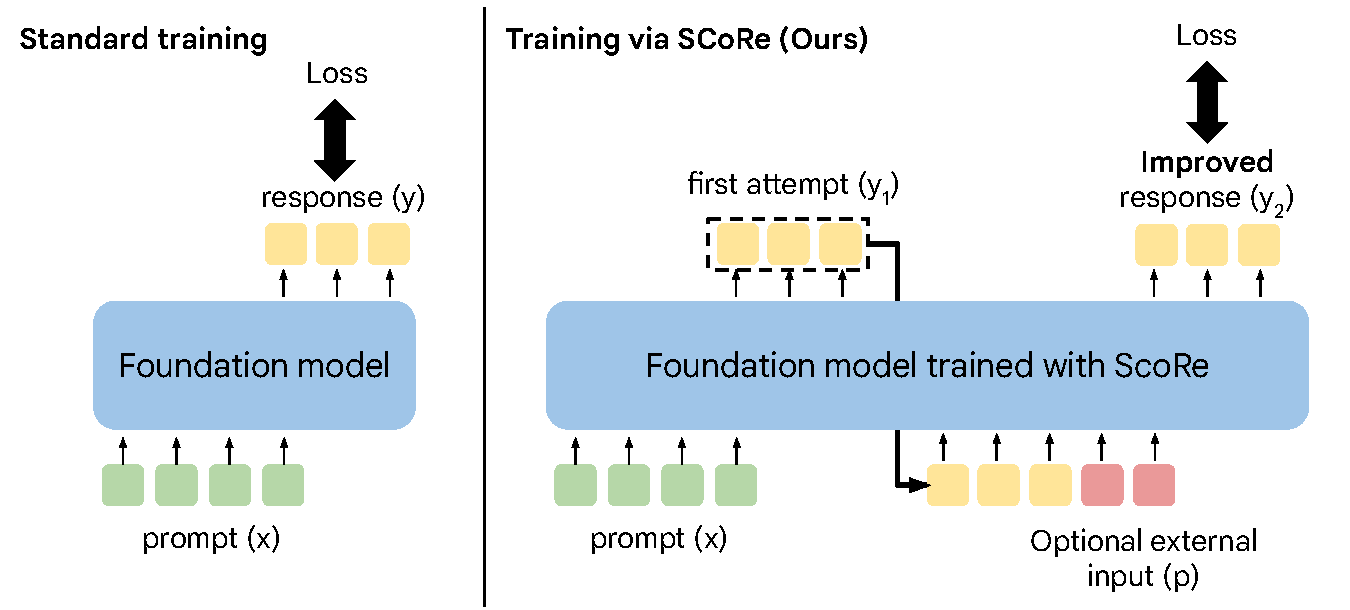
\includegraphics[width=0.7\linewidth]{assets/SCoRe_main_figure.pdf}
    \caption{\footnotesize{\textbf{The problem setting of self-correction.} \methodname{} trains a model to not just produce the best possible response, but instead aims to train the model to produce the best final response in the final attempt. In the second turn, extra input in the form of an instruction asking the model to correct itself or model-generated may be provided.}}
    \label{fig:problem_setup}
\end{figure}





